%Section3.tex

%%%%%%%%%%%%%%%%%%%%%%%%%%%%%%%%%%%%%%%%%%%%%%%%%%%%%%%%%%%%%%%%%%%%%%%%%%%%%%%%%
\section{Real root location}\label{S:three}
%
%
The remaining methods in  \texttt{RealRoots} are linear-algebraic any may be used to cont real zeroes of an ideal $I$ in $\RR^n$ according to
the sign of another polynomial, similar to Sylvester's Theorem~\ref{Th:Sylvester}.
We demonstrate how this may be used for real root location and remark om its applicability for other fields.

A symmetric bilinear form \defcolor{$S$} in a real vector space $R$ has two basic invariants, its rank \defcolor{$\rho(S)$} and signature
\defcolor{$\sigma(S)$}.
If we choose a basis for $R$ and thus a corresponding matrix $M$ representing $S$, then $M$ will be symmetric, and therefore 
diagonalizable with all $d\vcentcolon = \dim(R)$ eigenvalues real.
The rank $\rho(M)$ of $M$ is its number of nonzero eigenvalues, and its signature  is the difference
\[
\sigma(M)\ \vcentcolon =\ \#\{\mbox{positive eigenvalues of $M$}\}
\ -\ \#\{\mbox{negative eigenvalues of $M$}\}\,.
\]
Sylvester's Law of Inertia asserts that the rank and signature are independent of the choice of basis, and therefore are invariants of the
symmetric form $S$.

Let $\KK$ be any field, let $I\subset\KK[x_1,\dotsc,x_n]$ be a zero-dimensional ideal, and set
$\defcolor{R}\vcentcolon=\KK[x_1,\dotsc,x_n]/I$, an  Artinian ring.    
For $f\in R$ (or in $\KK[x_1,\dotsc,x_n]$) multiplication by $f$ induces an endomorphism $m_f$ of $R$ as in Section~\ref{S:two}.
For $h\in R$ (or in $\KK[x_1,\dotsc,x_n]$) we define the symmetric bilinear \demph{trace form} $S_h$ on $R$ by
$S_h(f,g)\vcentcolon= \mbox{trace}(m_{fgh})$.
The significance of the trace form is the following theorem.

%%%%%%%%%%%%%%%%%%%%%%%%%%%%%%%%%%%%%%%%%%%%%%%%%%%%%%%%%%%%%%%%%%%%%%%%%%%%%%%%%%%%%%%%%%%%%%%%%%%%
\begin{theorem}[\protect{\cite[Thm.\ 4.72]{BPR}}]
  Suppose that $\KK$ is a subfield of $\RR$ and $I\subset\KK[x_1,\dotsc,x_n]$ is a zero-dimensional ideal with zeros
  $\calV(I)\subset\CC^n$.
  For $h\in\KK[x_1,\dotsc,x_n]$, the rank and signature of the trace form $S_h$ satisfy
  %
  \begin{eqnarray}
    \rho(S_h)&=&    \label{Eq:traceCount}
      \#\{ z \in \calV(I) \mid h(z)\neq 0\}   \\
    \sigma(S_h)&=&
        \#\{ z \in \calV(I)\cap\RR \mid h(z)> 0\} \ -\  \nonumber
        \#\{ z \in \calV(I)\cap\RR \mid h(z)< 0\} \,.
  \end{eqnarray}
\end{theorem}
%%%%%%%%%%%%%%%%%%%%%%%%%%%%%%%%%%%%%%%%%%%%%%%%%%%%%%%%%%%%%%%%%%%%%%%%%%%%%%%%%%%%%%%%%%%%%%%%%%%%


We demonstrate how this may be used for real root location and comment on its applicability over other fields.
 this for the ideal $I$ of Section~\ref{S:two}.
Let
\[
 {\color{myblue}f\ \vcentcolon=\ 5-3x^2-3y^2+x^2y^2}\,,
\ \quad
  {\color{myred}g\ \vcentcolon=\ 1+2xy-4xy^2+3x^2y}\,.
\]
These define two curves in $\RR^2$, shown in Figure~\ref{F:two}.
%%%%%%%%%%%%%%%%%%%%%%%%%%%%%%%%%%%%%%%%%%%%%%%%%%%%%%%%%%%%%%%%%%%%%%%%%%%%%%%%%%%%%%%%%%%%%%%%%%%%
\begin{figure}[htb]
  \centering
  \begin{picture}(168,120)(-3,0)
     \put(0,0){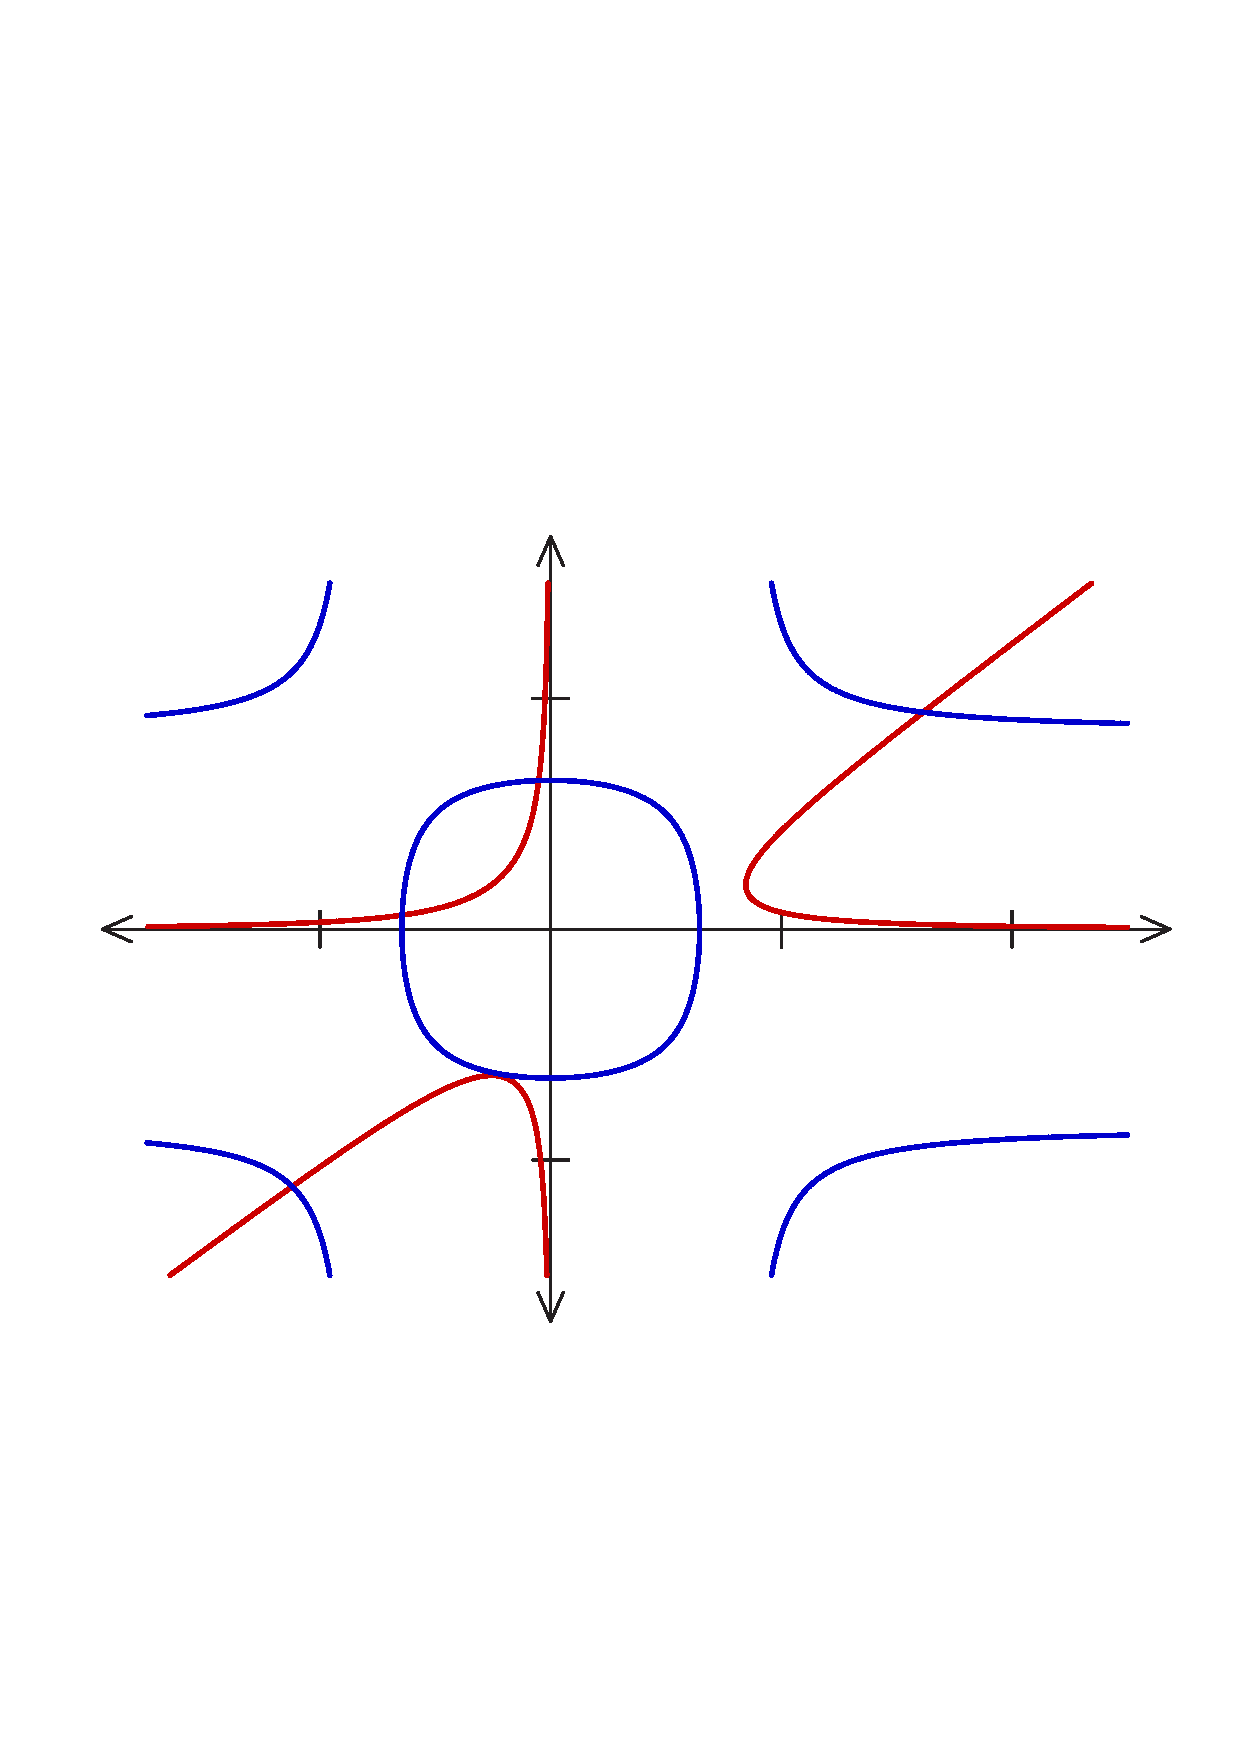
\includegraphics[height=120pt]{pictures/TwoCurves}}
     \put( 2,4){{\color{myred}\small$f$}}
     \put(60,100){{\color{myred}\small$f$}}     \put(152,110){{\color{myred}\small$f$}}
     \put(-2,90){{\color{blue}\small$g$}}     \put(158, 90){{\color{blue}\small$g$}}
         \put(88,80){{\color{blue}\small$g$}}
     \put(-2,26){{\color{blue}\small$g$}}     \put(158,26){{\color{blue}\small$g$}}
    \put(22,48){\small$-2$}    \put(101,48){\small$2$}   \put(135,48){\small$4$}
    \put(72,23){\small$-2$}    \put(72,92){\small$2$} 
  \end{picture}
  %%%%%%%%%%%%%%%%%%%%%%%%%%%%%%%%%%%%%%%%%%%%%%%%%%%%%%%%%%%%%%%%%%%%%%%%%%%%%%%%
  \caption{Two real curves}
  \label{F:two}
\end{figure}
%%%%%%%%%%%%%%%%%%%%%%%%%%%%%%%%%%%%%%%%%%%%%%%%%%%%%%%%%%%%%%%%%%%%%%%%%%%%%%%%%%%%%%%%%%%%%%%%%%%%
While they have eight complex points in common,
%
%  Call traceCount(I) or traceNumber ?
%
only four are real.
%
%  Call traceReal(I)    
%
%
\begin{leftbar}
\verbatiminput{examples/traceCounting.txt}
\end{leftbar}
%
We saw this in Section~\ref{S:two}, following \texttt{o21}.
Thus the possible tangency that we see in the third quadrant is only a near miss.

Let us see this in another way, consider the signature of $S_y$,
%
\begin{leftbar}
\verbatiminput{examples/traceSignature.txt}
\end{leftbar}
%
Which appears to be wrong (it should be 2, I think).

%Trace form is Thm 4.72 in BPR
%
%Sylvester's theorem  is Thm. 2.55 in BPR
%

